%%%%%%%%%%%%%%%%%%%%%%%%%%
\chapter{LITERATURE REVIEW} \label{chap:2}
%%%%%%%%%%%%%%%%%%%%%%%%%%
\def\JPC{{\it J. Phys. C : Solid State Phys\ }\/}
\def\JCP{{\it J. Chem. Phys.\ }\/}
\def\JCOM{{\it J. Comput. Phys.\ }\/}
\def\JPF{{\it J. Phys. F : Metal Phys\ }\/}
\def\JPCM{{\it J. Phys. Condens Matter\ }\/}
\def\PR{{\it Phys. Rev.\ }\/}
\def\PRL{{\it Phys. Rev. Lett.\ }\/}
\def\JMMM{{\it J. Magn. Mag. Mater\ }\/}
\def\APL{{\it Appl. Phys. Lett.\ }\/}
\def\ESSL{{Electrochem. and Solid State Lett. }\/}
\def\RMP{{\it Rev. Mod. Phys.\ }\/}
\def\RPP{{\it Rep. Prog. Phys.\ }\/}

% % % % % % % % % % % % % % % % % % % % % % % % % % % % %

We present the review of relevant literature in this chapter. We go through the literature related to MD simulations, measurements of thermodynamics and transport properties (especially, diffusion coefficients, mobility, friction coefficients, free energy of solvation )  methane and different studied system in water. We also discuss the effect of solvents on free energy of solvation of lighter alkanes in different solvent environment.  
%%%%%%%%%%%%%%%%%%%%%%%%%%
\section{Structure and dynamics properties of methane and various gases in water}
%%%%%%%%%%%%%%%%%%%%%%%%%%
MD simulations were first conducted in the 1950s~\citep{Haile1992}. These methods are becoming more prevalent due to ongoing computational enhancements and members of the research community are turning to these methods with new questions and problems. Given a set of initial conditions, MD simulations can be used to compute the movement of individual molecules under the action of forces. If it is
possible to simulate motion at the molecular level, then it should be possible to use MD
simulation to study molecular diffusion of  gases in water. Diffusion is fundamental for transport of matter and for ionic conduction in disordered materials~\citep{harmandaris2007, adhikari2004}. The kinetics of many micro-structural changes that occur during preparation, processing and heat treatment of materials include diffusion, typical examples are nucleation of new phases, diffusive phase transformation precipitation and dissolution of a second phase, homogenization of alloys, recrystallization and thermal oxidation~\citep{mehrer2007}. The application of diffusion is on doping during fabrication of microelectronic devices, the operation of solid electrolytes for batteries and fuel cells, surface hardening of steel through carburisation or nitridation etc.~\citep{mehrer2009}.

The first attempt to measure self-diffusion (the most basic diffusion process) was done by physico-chemist George Karl Von Hevesy who studied self-diffusion in liquid~\citep{groh1920} and in solid lead~ \citep{groh1921} by using a natural radioisotope  $^{210}Pb$ and $^{212}Pb$ of lead. From the pioneering work of Alder and Wainwright~\citep{PhysRevLett1967, alder1970}  the simulation of diffusion coefficient has been an area of continuous research. The equations of Fick, the statistical interpretation of diffusion coefficient by Einstein and Smoluchowski and the Boltzmann-Matano method for concentration dependent diffusion coefficients opened the way for new experimental techniques~\citep{mehrer2009}. Experimental study of Diffusion process can be done by different methods. Electron-Spin Resonance (ESR), Dynamic Light Scattering (DLS) and Nuclear magnetic resonance (NMR) are some famous techniques which enable to study diffusion coefficient. These methods are expensive and hard to handle. Now study of diffusion coefficient can be done by using computer simulation technique and these are cheaper and effective way to proceed~\citep{Allen1989}. Now, there is a magnificent increase in the application of computer modeling and simulation method in different areas of research~\citep{adhikari2003, adhikari2002, Leach2001} and to study the diffusion process ~\citep{harmandaris2007}. The study of the diffusion  have been done using
molecular dynamics simulation technique ~\citep{Thapa2013, dahal2012}. Rahman (1971) considered 216 rigid water molecules to examine the structural and kinetic behavior of liquid water at $34.3$ $^{\circ}$~ \citep{rahman1971}. Malenkov et al. ~\citep{malenkov2009, malenkov2011} studied the physical, structural and dynamical properties of liquid water and ice. Malenkov considered a huge system containing 3456 water molecules to study the correlation coefficient. In the present days, computer modeling and simulation method have been widely used in the different areas of research \citep{bird2015introductory}. Classical Molecular dynamics simulation is one of computer simulation technique for computing the equilibrium transport properties of classical many-body system. Due to the availability of the open source packages like GROMACS~\citep{Gromacs-manual}  and the different experimental techniques Ringbom apparatus~\citep{smith1955experimental}, Diaphragm cell, Infinite Couple, Taylor Dispersion, Nuclear Magnetic resonance \citep{cussler2009}  the study of diffusion process is familiar in large scientific family. 

MD simulation has been used to study the diffusion of nitric oxide in liquid water~\citep{zhou2005molecular} and  the aqueous  diffusivities and solubilities of nitric oxide were determined by using chemiluminescence detector to measure time-dependent fluxes across stagnant liquid films confined between  polydimethylsiloxane membranes~\citep{zacharia2005diffusivity}. The polymorphic sensors were used for the in situ monitoring of nitric oxide release and diffusion from the endothelial cell through the muscle cells found in rabbit aorta and the experimental data was compared with Fick's equation for linear diffusion~\citep{malinski1993diffusion}. The experimental
study of diffusion process for dissolved neon, krypton, xenon, carbon monoxide and nitric oxide have been measured in water by following the rate of collapse of small bubbles in gas-free water~\citep{wise1968diffusion}. Also diffusion of hydrogen, carbon monoxide, and water in liquid n-alkanes at elevated temperatures and pressures~\citep{makrodimitri2011molecular}, where n-alkanes were modeled based on the united-atom Transferable Potentials for Phase Equilibria (TraPPE-UA) and simulation runs were on the order of 30 nanoseconds (ns). Mutual diffusion coefficients for gas mixtures of ethane/nitrogen and n-pentane/nitrogen have been estimated using MD simulation and compared to measured values~\citep{chae2011mutual}. Diffusion coefficients of heptane isomers in nitrogen in the range of 500 to 1000 K was measured by MD simulation ~\citep{chae2011mutual}, where results were compared to estimates from Chapman-Enskog (CE) theory and the all-atom Optimized Potentials for Liquid Simulations (OPLS-AA)
was used to describe molecular interactions and simulation runs were on the order of
14 ns.

\begin{sloppypar}
The diffusion coefficients of short n-alkane molecules in water for wide ranges of temperatures and pressures have been repeatedly measured experimentally and from numerical simulations during the last 3-4 decades~\citep{sachs1998diffusional, lu2006situ, price2000self, jahne1987measurement, maharajh1973temperature, witherspoon1969correlation}. The experimental values of binary diffusion coefficients of alkane-water mixture have been obtained by Wise and Houghton~\citep{wise1966diffusion}, by using the rate of collapse of small bubbles in gas free water. Also, Witherspoon and Saraf~ \citep{witherspoon1965diffusion}, have been obtained by using the capillary cell method. Most recently,
the diffusion coefficients of CH4 in H2O for temperatures up to 473 K and pressures up to
40 MPa have been measured by Guo et al.~\citep{guo2013situ} by means of Raman
spectroscopy and Michalis et al. ~\citep{michalis2016molecular} calculated the diffusion coefficients of light n-alkanes in water over a wide range of temperature and pressure by numerical simulation method. The calculated diffusion coefficients agree well to some of the earlier experimental results but these results are forcefield parameter dependent. The authors in ~\citep{michalis2016molecular}
have used TraPPE~\citep{martin1998transferable} force field for the representation of n-alkane. The TraPPE is a united atom model in which methyl (CH 3 ) and methylene (CH 2 ) groups of alkanes are represented as two point particles (pseudo-atoms along the alkane chain connected with bonds of fixed length) and positively charged hydrogen atoms are merged with an electronegative carbon atom in each group. All groups have zero charge and hence Coulomb interactions are excluded. The number of dihedral (or torsion) interaction constants is less and therefore the parametrization becomes simpler. The total energy also becomes lower. This model seems less realistic though it takes the least computational cost. On the other hand, OPLS-AA~\citep{kaminski2001evaluation} is an all-atom model for alkane that includes Coulomb interaction and the changes in the distribution of the electron density (due to the polar covalent bonds inside molecules) create non-zero atomic charges. Due to explicit hydrogen atoms, OPLS-AA uses a more complex form of dihedral interaction and there is more steric clashes between hydrogen atoms on neighboring molecules. There is both Coulomb and Lennard-Jones interactions. The Coulomb interaction and the more complicated torsion should give the difference in the physical properties though it needs the more computational cost. All-atom model is more realistic than that of united atom model, so it is better to use OPLS-AA to reproduce and predict transport properties of alkanes~\citep{moultos2016atomistic, kondratyuk2015relaxation}. Such discrepancies in previous experimental works and forcefield parameter dependent of diffusion coefficients calculated by numerical simulation motivated us to carry out a computational work by different forcefield to study the diffusion phenomena of alkane in water. Our results obtained from simulation also can be used as a crude reference for any further studies of diffusion in complex fluid mixtures and improve our understanding of hydrocarbons and other more complex biological macromolecules in water.
\end{sloppypar}


\section{Diffusion and ion mobilities of alkali and halide ions in water}
 Chong and  Hirata~\citep{chong1999dynamics} presented a molecular theory for investigating the dynamics of ions in polar liquids. The theory was based on the interaction-site model for molecular liquids and on the generalized Langevin equation combined with the mode-coupling theory. They studied the velocity autocorrelation function, diffusion and friction coefficients of ions in water at 25 $^{\circ}$C and at infinite dilution. Mohammad et al.~\citep{mohammad2015diffusion} calculated the diffusion Coefficient of iodide ion  through cyclic voltammetric  technique. The contribution of (a) the fractal surface of  the electrode, and (b) possible involvement of subsequent chemical reaction (EC) to the peak current  affecting the diffusion coefficient were analyzed. Koneshan et al.~\citep{koneshan1998solvent} calculated the mobilities  of the metal cations $\mathrm{Li^{+}}$, $\mathrm{Na^{+}}$, $\mathrm{K^{+}}$, $\mathrm{Rb^{+}}$, $\mathrm{Cs^{+}}$,  $\mathrm{Ca^{++}}$ and the halides $\mathrm{F^{-}}$, $\mathrm{Cl^{-}}$, $\mathrm{Br^{-}}$, and  $\mathrm{I^{-}}$  at infinite dilution by molecular dynamics simulation using the SPC/E model for water at 25 $^{\circ}$C  and a reaction field for the long-range interactions. The ion mobilities show the same trends as the experimental  results with distinct maxima for cations and anions. The mobilities of  $\mathrm{Li^{+}}$, $\mathrm{Na^{+}}$, $\mathrm{K^{+}}$ $\mathrm{Rb^{+}}$ and $\mathrm{F^{-}}$  increase on discharge, whereas Cl, Br, and I have smaller mobilities  than the corresponding anions. Koneshan et al.~\citep{koneshan1998friction} estimated the diffusion coefficients of ions and of uncharged solutes in aqueous solution at 25 $^{\circ}$C and at  infinite dilution are studied by computer simulation using the SPC/E model for water and solute-water potentials  employed in their previous work~ \citep{koneshan1998solvent}. The mobilities of  the ions calculated from the diffusion coefficients pass through a maximum as a function of ion size, with  distinct curves and maximums for positive and negative ions in qualitative agreement with experiment. Further, Lynden-Bell and Rasaiah ~\citep{lynden1996mobility}  presented  some results from a simulation study of the mobility and solvation of ions and uncharged molecules in aqueous solution in smooth cylindrical channels at room temperature. This ideal system provided a reference system with which to compare the behavior of water and ions in real porous materials such as zeolites, bucky tubes, and biological channels.  Lee and   Rasaiah ~ \citep{lee1994molecular}  described a series of molecular dynamics simulations performed on model cation-water systems  at 25 $^{\circ}$C representing the behavior of $\mathrm{Li^{+}}$, $\mathrm{Na^{+}}$, $\mathrm{K^{+}}$ $\mathrm{Rb^{+}}$ and $\mathrm{Cs^{+}}$ in an electric field of 1.0 V/nm  and in its absence. The TIP4P model was used for water and TIPS potentials were adapted for the  ion-water interactions. The structure of the surrounding water molecules around the cations was found to be independent of the applied electric field. Lee and   Rasaiah~ \citep{lee1996molecular}  presented results of computer simulations of the mobilities of the alkali metal ions ($\mathrm{Li^{+}}$, $\mathrm{Na^{+}}$, $\mathrm{K^{+}}$ $\mathrm{Rb^{+}}$ and $\mathrm{Cs^{+}}$) and the halides ($\mathrm{F^{-}}$, $\mathrm{Cl^{-}}$, $\mathrm{Br^{-}}$ and  $\mathrm{I^{-}}$) 25 $^{\circ}$C using the SPC/E model for water and ion-water parameters fitted to the binding energies of small clusters of ions. A simple truncation of the ion-water and water-water potentials was used, and the mobilities calculated from the mean square displacement and the velocity autocorrelation functions, respectively, were found to be in good agreement with each other. 
 
 \begin{sloppypar}
 The dynamic and energetic properties of the alkali and halide ions were calculated using molecular dynamics (MD) and free energy simulations with various different water and ion force fields including our recently developed water-model-specific ion parameters. The properties calculated were activity coefficients, diffusion coefficients, residence times of atomic pairs, association constants, and solubility. Through calculation of these properties, we can assess the validity and range of applicability of the simple pair potential models and better understand their limitations. Due to extreme computational demands, the activity coefficients were only calculated for a subset of the models. The results qualitatively agree with experiment. Calculated diffusion coefficients and residence times between cation-anion, water-cation, and water-anion showed differences depending on the choice of water and ion force field used~\citep{joung2009molecular}.
\end{sloppypar}

%%%%%%%%%%%%%%%%%%%%%%%%%%
\section{ Light Alkane in  polar and amphiphilic environment}
%%%%%%%%%%%%%%%%%%%%%%%%%%
In this work simulations of solvation of alkanes in two different solvents are done. As a solvent
we used water as a polar substance and methanol as amphiphilic substance. In the literature
there are  many articles dealing with  solvation of alkanes in water. For methanol as a solvent not even one article was found. 

\begin{sloppypar}
Hydrophobicity can be understood in terms of disaffinity of oil with water ~\citep{Southall2002}. This simple physical observation, however, carries a significant meaning in chemical and biological processes. Protein folding, ligand-protein and protein-protein binding, membrane and micelles formation  are some of the examples where the hydrophobic effect plays a key role. Protein folding, a familiar biological process, is the consequence of complex combination of forces/contributions, few of which are electrostatic, hydrogen bonding, van der Waals interactions and some other intrinsic properties \citep{Dill1990}. Folded proteins at room temperature are marginally stable, and thus even a small change in any contributing factor/s may alter their structure and stability ~\citep{Dill1990}. Because of its significance in a number of research areas, more importantly in chemical, biological and pharmaceutical sciences~\citep{Djikaev2016}, hydrophobicity in aqueous medium has been the subject of curiosity for researchers of diverse field via experiments~\citep{Crovetto1982}, theoretical analysis ~\citep{Pratt1980} and computer simulations ~\citep{Guillot1993}, since more than two centuries. 
\end{sloppypar}

An experiment performed by Benjamin Franklin has been considered as the first reported work of hydrophobicity (in 1773) where a drop of oil was poured into water~\citep{Tanford2004}. Rayleigh almost a century later estimated the size of a molecule by assuming single layer of oil film above water based on the property of disaffinity in between two liquids ~\citep{Tanford2004}. In case of biological molecules like proteins, made up of a large number of aminio acids and side chains, the native structure is found in folded state \citep{Tanford1997, Alberts2002}. The role of hydrophobicity in protein folding was introduced by Kauzmann at the time when details of protein structure and mathematical algorithms were not developed~\citep{Kauzmann1959}. The author further introduced about the primary, secondary and tertiary protein structures.  The amphiphilic properties of proteins and soaps, where the hydrophobic and hydrophilic groups are available in the same molecule, were however already recognized ~\citep{Tanford1997}. The precise study (with numerics) of oil and surfactants on water were studied by Langmuir in 1917 ~\citep{Langmuir1917}. In amphiphilic molecule, the hydrophobic (non-polar) groups of hydrocarbon (which are hidden in the native protein structure) were found to be exposed to water upon their denaturation in 1941 \citep{Bull2009}. The prediction was later verified by X-rays experiments in micelles and proteins, and observed that  polar and nonpolar groups were aggregated at the surfaces and interior of the structures respectively.  

As we discussed before, the disaffinity of water for oil is controlled through various interactions.
Surprisingly, no repulsive interactions in between two liquids exist in such disaffinity, rather the attractive forces in between like molecules, water with water and oil with oil, have been noticed~\citep{Southall2002}. Among the attractive hydrogen bonding and dispersion interactions, hydrogen bonding in between water molecules is stronger and dominant over the dispersion interactions in oil \citep{Pauling1960}. Because of the dipolar and nonpolar groups, and helix-coil transitions in proteins, electrostatic and intrinsic molecular interactions are also important in their conformational changes and ion-pairing interactions~\citep{Anufrieva1967}. The electrostatic interactions are the function of ionic-strength, their positions and dynamics, and PH value (total charge) of the total system ~\citep{Gitlin2006}. The effect of changes in acidity and basicity (changes in charge concentration) has been described in terms of non-specific electrostatic repulsion which is dominant at higher concentration and helps to destabilize the folded protein~\citep{Tanford1961}. The ion-paring interactions (where a charge is shielded by oppositely charged aminoacids), on the other hand, are effective at lower ionic concentration and support for protein stability~\citep{Dill1990}. Comparing these two contradictory effects, the ionic shielding gets saturated beyond certain concentration and the pairing (specific charge) interaction becomes less important. 

The distance dependent interactions (in between interacting units), which were first introduced during the middle of twentieth century~\citep{Hill1960}, are categorized as long-ranged and short-ranged. The interaction is long-ranged if the total energy varies with $r^{-p}$, for $p \leq 3$. It is said to be short-ranged if $p > 3$. The ion-ion/ion-dipole type, and  Lennard-Jones type of interactions are the examples of as long-ranged and  short ranged interactions respectively. Go and Taketomi in 1978~\citep{Go1978}, by using Monte-Carlo simulations, further explained the particular role of distance dependent interactions: (i) long-ranged for stabilization and (ii) short-ranged for rate of folding and unfolding during the changes in protein conformations. Local and non-local were also categorized depending upon whether the units are topologically near or far-positioned ~\citep{Go1979, Abkevich1995}.

\begin{figure}[h!]
\begin{center}
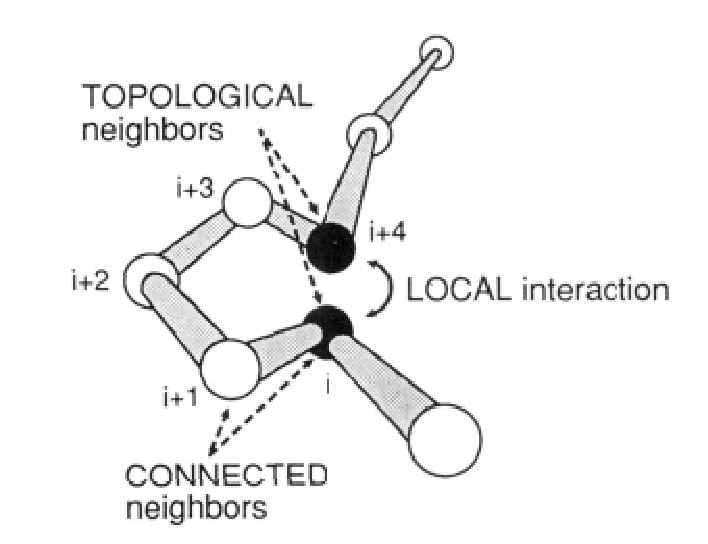
\includegraphics[width= 0.23\textheight]{Chapter2/local_protein.eps}
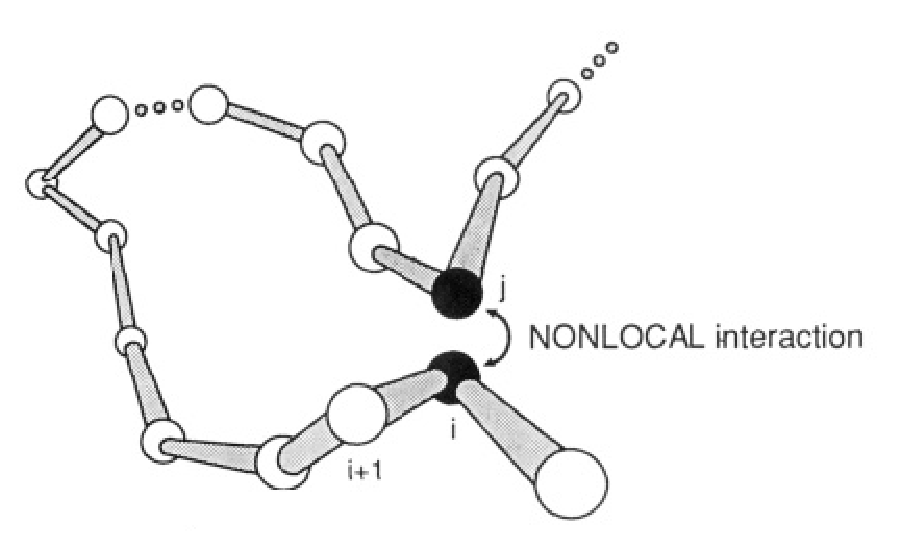
\includegraphics [width= 0.23\textheight]{Chapter2/nonlocal_protein.eps}
\caption[Local and non-local interactions.]{Local and non-local interactions. Polymer residues and their interactions are defined as local and non-local depending upon immediate and topological neighbors, respectively~\citep{Dill1990}.
}
\label{local-nonlocal} 
\end{center}
\end{figure}

Protein stability and their configurations may change with the variation in temperature, pressure and composition of solvent-constituents (salt and other organic solvents) around them ~\citep{Djikaev2016}. The stability, in general, decreases with increasing temperature due to increase in entropy and free energy, which however, might be decreasing with decreasing temperature in some cases. This unexpected phenomenon is recognized as {\it cold denaturation}~\citep{Privalov1988, Southall2002}. Proteins are thus marginally stable for a certain range of temperature and, unstable elsewhere. Furthermore, hydrophobicity is driven by entropy at low temperature and enthalpy at high temperature~\citep{Southall2002}. 

In biological creatures, protein activities are affected by their solvent environment. The effect of 
aqueous solution in model protein systems are thus important to understand in atomistic level. For a nonpolar solute in water, it is noticed that water forms a clathrate-like shell and does not waste its hydrogen bonding by pointing towards solutes on the cost of strong (hydrogen) 
bonding with another water. Frank and Evens introduced this concept as {\it iceberg model}~\citep{Frank1945}, where the ordered water structure surround protein keeping nonpolar amino acids at the inner part so that they do not directly meet water. The nonpolar residues come up to the surface only after protein denaturation~\citep{Dill1990}. The size and nature of interacting particles are also found to be important in hydrophobicity, and the stability of protein structure~\citep{Djikaev2016}. The effect of molecular-size of both the solute and solvents on hydrophobicity have been discussed by using the concept of free energy and other thermodynamic parameters. Lucas computed the changes in free energy due to transfer of nonpolar solutes from gaseous states to water and other solvents as a function of solvent's molecular dimension~\citep{Lucas1976}. The author and the later works~\citep{Lee1985} proposed that the increase in free energy due to insertion of nonpolar molecules into water was because of 
requirement of appropriate cavity to adjust the solute particles. Larger the molecular size of solvents create larger the cavity, and easier to adjust the solutes in the cost of small changes in free energy. Since the water molecules are among the smallest solvent molecules, it can be predicted that the solubility of nonpolar solutes in water is low (indicating higher hydrophobicity). The size-effect of solute particles has also been searched on the basis of solvation energy ~\citep{Chan1991, Mcauliffe1963}. Although there are some controversial views for selecting more precise  parameter, whether molar volume or solvent-accessible surface area of solute to calculate the solubility of hydrocarbons in water~\citep{Parker1963, Frank1966, Reynolds1974}, it could be appreciated that free energy of solvation increases with the solute dimension (due to the requirement of larger cavity in solvent). The correct formulation for the proportionality, however,
requires molecular shape and geometry ~\citep{Lazaridis2000}.

\begin{sloppypar}
More examples of organic solvents to study their response on protein conformations, denaturation, stabilization and crystallization through hydrophobic effect have been searched. Addition of methanol in aqueous solution of peptide BBA5 has been found to increase the size of the  hydrophobic core and weaken the hydrophobic effect~\citep{Hwang2011}. Similar effect of acetoitrile (AN), where the OH group of methanol is replaced by CN group, is seen in case of lysozome (protein) immersed water-AN mixture. When the concentration of AN crosses 40~\% (by weight), hydrophobic effect weakens on the cost of increasing peptide-peptide hydrogen bonds \citep{Gekko1998}. The order of solubility of small non-polar side chains increases from AN towards methanol and then ethanol. Urea and guanidium chloride (GdmCl), on the other hand, have little effect in hydrophobic association for the denaturation of protein molecules \citep{O'brien2007}. 
\end{sloppypar}

Hummer et al., by using computational method, estimated the effect of surrounding pressure on stability of model system for protein structure~\citep{Hummer1998}. Unlike the usual convention of transfer of solute particles in water, the authors proposed that the water molecules enter into the protein interior due to increasing pressure which leads to the denaturation of protein structure. The results show decreasing methane-methane (contact) interactions and increasing desolvation barrier during the elevated pressure. At higher pressure, the energy cost of forming cavity increases, and destabilize the contact configurations with respect to solvent separated configurations. The role of structure making and structure breaking around the ion-cores in different solvents was studied by Ding et al.~\citep{Ding2014}. In this context, a comparative study of solvent-effects will be meaningful for the better understanding of biochemical processes in living beings. We consider first four light alkanes   interactions in water and methanol; water as a polar molecule and methanol as an amphiphilic molecule, to model stability of protein structure in different solvents. 


The hydrophobic hydration and interaction of apolar Lennard-Jones solutes as a  function of temperature in the range between 275 and 375 K along the 0.1 MPa isobar was investigated for five different popular rigid water models (SPC, SPCE, TIP3P, TIP4P, and TIP5P) using molecular dynamics simulations~\citep{paschek2004temperature}.  A detailed comparison of computational efficiency and precision for several free energy difference methods were presented  and the analysis included both equilibrium and nonequilibrium approaches, and distinguishes between unidirectional and bidirectional methodologies~\citep{ytreberg2006comparison}. The free energy of hydration of 15 amino acid side chain analogs derived from the OPLS-AA parameter set with the TIP3P, TIP4P, SPC, SPC/E, TIP3P-MOD, and TIP4P-Ew water models were estimated  to examine the accuracy of a range of common water models used for protein simulation for their solute/solvent properties~\citep{shirts2005solvation}. Free energy of transfer of methylamine, octylamine, methanol, and octanol from water phase to sodium dodecyl sulfate (SDS) micelle and Free energy of transfer from water phase to a SDS micelle core  for a series of hydrophobic solutes originally immiscible with water  have been calculated by thermodynamic integration method combined with molecular dynamics calculations~\citep{fujimoto2010molecular,fujimoto2012molecular}. The expanded ensemble method ~\citep{lyubartsev1992new} has been  applied to calculate solvation free energies for methane disolved in water at infinite dilution and at finite concentration and for several of monovalent anions and cations in aqueous solution\citep{lyubartsev1996calculations}. The first complete description of the solution thermodynamics of a series of linear, branched, and cyclic alkanes in water, including the enthalpy and entropy changes in addition to the solvation free energies have been reported  by computer simulations\citep{gallicchio2000enthalpy}. They have also obtained a complete thermodynamic description of the solvation of the associated alkane cavities.

We use method of classical molecular dynamics as the computational technique whose history starts from the fifties of twentieth century~\citep{Alder1957}. Assuming the particles as hard spheres
with elastic collision between them, Alder and Wainwright studied the dynamics of liquid molecules during late fifties \citep{Allen1989} by using the techniques of computer simulations. The development of MD passes through the Lennard Jones model in 1964 \citep{Rahman1964} and 
then towards the dynamics of larger molecules \citep{Kremer2003} upon the development of digital computers. In the present work, we use GROMACS ( GROningen MAchine for Chemical Simulations) as the computing software~\citep{Gromacs-manual} whose details will be discussed in section 3. 


